\chapter{Algorytmy regulacji predykcyjnej}
Do lat 70. ubiegłego wieku warstwa regulacji bezpośredniej w warstwowej strukturze sterowania (Rys. \ref{warstwy}) zapewniała przede wszystkim niezawodność \cite{120}. Dominowały wówczas algorytmy PID, natomiast rozwój optymalizacji postawił nowe wymagania przed układami regulacji \cite{160}. Okazało się bowiem, że skuteczna regulacja podczas optymalizacji punktu pracy przynosi duże korzyści ekonomiczne. To można było osiągnąć dzięki wprowadzeniu nowej grupy algorytmów - algorytmów regulacji predykcyjnej z przesuwnym horyzontem, zwanym też zasadą sterowania repetycyjnego \cite{160}. Pozwoliły po raz pierwszy rozwiązać problem uwzględnienia ograniczeń sygnałów sterujących.

\begin{figure}[h!]
\centering
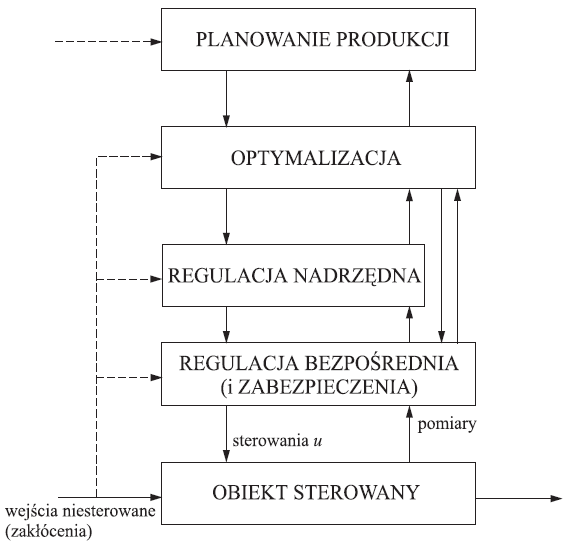
\includegraphics[width=0.5\textwidth]{pictures/warstwy}
\caption{Warstwowa struktura sterowania \cite{121}.}
\label{warstwy}
\end{figure}

W każdej chwili próbkowania, dysponując dynamicznym modele obiektu, pomiarami sygnałów procesowych oraz znaną lub założoną trajektorią wyjść zadanych wyznaczana jest sekwencja przyszłych wartości sygnału sterującego przez optymalizację funkcji celu zdefiniowanej na horyzoncie predykcji \cite{40}.

Najczęściej spotykana postać funkcji kryterialnej wygląda następująco:
\begin{equation}
J(k) = \min_{\Delta U(k)} \quad \{\sum_{p=1}^N (y^{zad}(k+p|k) - \hat{y}(k+p|k))^2 + \lambda \sum_{p=0}^{N_u} (\Delta u(k+p|k))^2\}
\end{equation}

przy ograniczeniach:

\begin{equation}
\begin{aligned}
u^{min} \quad &\leq& u(k+p|k) \quad &\leq& u^{max} \\
-\Delta u^{max} \quad &\leq& \Delta u(k+p|k) \quad &\leq& \Delta u^{max} \\
y^{min} \quad &\leq& \hat{y}(k+p|k) \quad &\leq& y^{max}
\end{aligned}
\end{equation}

\newpage

Wskaźnik jakości dostarcza informacji jakie wyniki powinien generować algorytm: uchyby regulacji muszą być jak najmniejsze, natomiast przyrosty sterowania nie powinny przyjmować dużych wartości, a ponadto korygowane są tzw. parametrem kary. Wyeliminowanie tego składnika ($\lambda = 0$) generuje przebiegi sygnału sterującego o dużych amplitudach i przyrostach, często niemożliwych do fizycznej realizacji. \\
Ograniczenia nałożone na sygnał sterujący związane są z uwarunkowaniami technologicznymi urządzeń wykonawczych, natomiast ograniczenia na sygnały wyjściowe służą spełnieniu norm technologicznych, ekonomicznych, a także zyskujących na coraz większym znaczeniu ekologicznych. Ogólna zasada regulacji predykcyjnej została zaprezentowana na Rys. \ref{mpc}

\begin{figure}[h!]
\centering
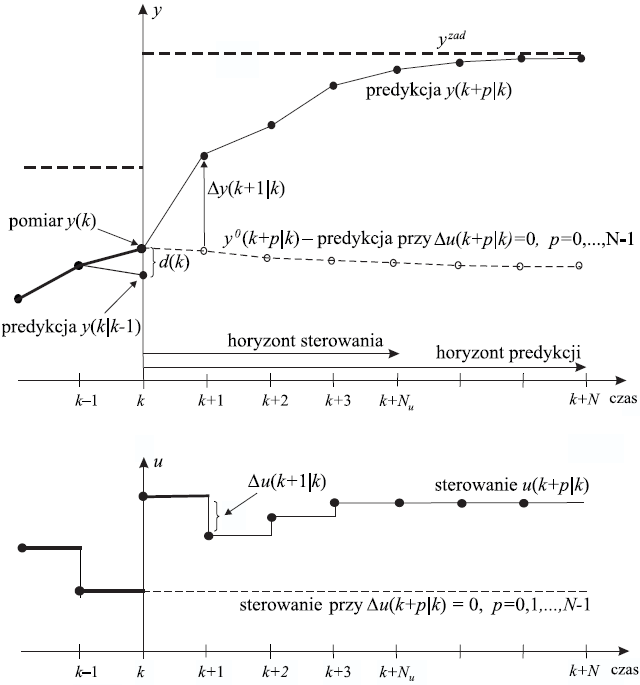
\includegraphics[width=0.65\textwidth]{pictures/mpc}
\caption{Zasada działania regulacji predykcyjnej \cite{122}.}
\label{mpc}
\end{figure}

Przedstawione przebiegi zawierają kilka istotnych aspektów, które warto opatrzeć komentarzem:
\begin{itemize}
\item[•] $y^{zad}$ - trajektoria sygnału zadanego, przyjmowana jako wartość stała na horyzoncie predykcji\footnote{Najczęściej zakładana jest stała trajektoria zadana, natomiast w niektórych dziedzinach, np. robotyka, dopuszcza się uwzględnienie zmian trajektorii zadanej w celu uprzedniego reagowania na jej zmiany.}
\item[•] $\Delta y(k+p|k)$ - prognozowana trajektoria odpowiedzi wymuszonej zależna tylko od zmiennych decyzyjnych - przyszłych przyrostów sterowań
\item[•] $y^0(k+p|k)$ - przewidywana odpowiedź swobodna, czyli wartości odpowiadające sytuacji, w której na całym horyzont predykcji $N$ utrzymywana byłaby wartość sterowania z chwili poprzedniej $u(k-1)$
\item[•] $\Delta u(k+p|k)$ - kolejne przyrosty sterowania wyznaczane na horyzoncie sterowania $N_u$
\end{itemize}

Na tej podstawie oraz korzystając z zasady superpozycji można zapisać:
\begin{equation}
y(k+p|k) = y^0(k+p|k) + \Delta y(k+p|k) \quad \quad p = 1 ... N
\end{equation}

\newpage

Zasada regulacji predykcyjnej jest dość uniwersalna co pozwoliło na wykształcenie kilku dominujących algorytmów, takich jak:
\begin{itemize}
\item[•] DMC (\textit{Dynamic Matrix Control}) - algorytm predykcyjny wykorzystujący model liniowy w postaci dyskretnych odpowiedzi skokowych
\item[•] GPC (\textit{Generalized Predictive Control}) - algorytm predykcyjny wykorzystujący model liniowy w postaci dyskretnych równań różnicowych
\item[•] MPCS (\textit{Model Predictive Control with State-space model}) - algorytm predykcyjny wykorzystujący w swoim opisie równania stanu
\item[•] MPHC (\textit{Model Predictive Heuristic Control}) - algorytm predykcyjny wykorzystujący model liniowy w postaci odpowiedzi impulsowej
\end{itemize}

Ze względu na praktyczną naturę algorytmu DMC do dalszych rozważań postanowiono przyjąć właśnie ten algorytm.

\section{DMC}
Algorytm DMC pierwszy raz został zaimplementowany przez grupę Shell Oil w latach \\ 70 XXw. Na tamten czas dało im to ogromną przewagę w branży petrochemicznej, a sam algorytm dzięki bezpośredniemu praktycznemu zastosowaniu stał się bardziej popularny. Algorytm ten zasadę swojego działania opiera na odpowiedzi skokowej, co wg autora \cite{120} stanowi jeden z najskuteczniejszych form identyfikacji obiektu. \\
Na Rys. \ref{step_response} przedstawiono przykład odpowiedzi skokowej na wymuszenie jednostkowe, zaprezentowane na horyzoncie dynamiki, czyli czas po którym wartość odpowiedzi skokowej można uznać za ustaloną, tj.
\begin{equation}
s_k = s_{k+1} = s_{k+2} = ... = s_D = s_{\infty}
\end{equation} 

\begin{figure}[h!]
\centering
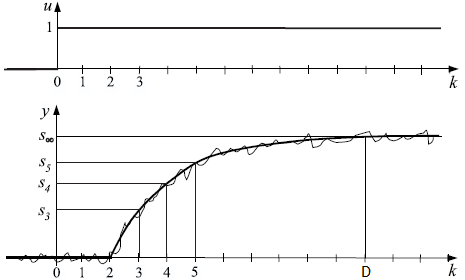
\includegraphics[width=0.75\textwidth]{pictures/step_response}
\caption{Odpowiedź skokowa \cite{123}.}
\label{step_response}
\end{figure}

Korzystając z zasady superpozycji, dla każdej chwili dyskretnej $k+p$, można zatem zapisać:

\begin{equation}
y^{mod}(k+p|k) = y^{mod}(0) + \sum_{j=1}^{k+p} s(j) \Delta u(k+p-j)
\end{equation}

\newpage

Z kolei wartość przewidywanej trajektorii wyjść można zapisać jako suma wartości modelu i~zakłócenia sprowadzonego do wyjścia:

\begin{equation}
\hat{y}(k+p|k) = y^{mod}(k+p|k) + d(k+p|k)
\end{equation} 

\noindent gdzie zakłócenie $d(k)$ jest równe różnicy między pomiarem wyjścia w chwili $k$, a wartością obliczoną z modelu w chwili $k-1$:

\begin{equation}
d(k) = y(k) - y^{mod}(k|k-1)
\end{equation}

\noindent natomiast ogólnie przejętą praktyką jest przyjmowanie modelu zakłóceń typu DMC, tj.

\begin{equation}
d(k+1|k) = d(k+2|k) = ... = d(k+N|k) = d(k)
\end{equation}

Takie założenia pozwalają na sformułowanie wyjściowej postaci trajektorii prognozowanej w algorytmie DMC:

\begin{equation}
\left\{
\begin{aligned}
\hat{y}(k+p|k) &= y^0(k+p|k) + \Delta y(k+p|k) \\
y^0(k+p|k) &= y(k) + \sum_{j=1}^k (s(j+p) - s(j))\Delta u(k-j)  \\
\Delta y(k+p|k) &= \sum_{j=1}^p s(j) \Delta u(k+p-j)
\end{aligned}
\right.
\label{prognoza}
\end{equation}

Zatem w ogólności można zapisać trajektoria prognozowana jest sumą odpowiedzi swobodnej i wymuszonej. Algorytm DMC występuje w wersji analitycznej bez oraz z rzutowaniem na ograniczenia oraz w wersji numerycznej, uwzględniającej te ograniczenia. 

\subsection{Algorytm DMC w wersji analitycznej}
Do sformułowania prawa regulacji w wersji analitycznej, w postaci wektorowej niezbędne jest zdefiniowanie wektorów postaci:

\begin{equation}
\begin{aligned}
Y^{zad} = \begin{bmatrix}
y^{zad}(k+1|k) \\ \vdots \\ y^{zad}(k+N|k)
\end{bmatrix}_{Nx1}, \quad
\hat{Y} = \begin{bmatrix}
\hat{y}(k+1|k) \\ \vdots \\ \hat{y}(k+N|k)
\end{bmatrix}_{Nx1}, \quad
\Delta U(k) = \begin{bmatrix}
\Delta u(k|k) \\ \vdots \\ \Delta u(k+N_u-1|k)
\end{bmatrix}_{N_ux1}
\end{aligned}
\end{equation}

\noindent Oraz macierzy wagowych:

\begin{equation}
\begin{aligned}
\Psi = \begin{bmatrix}
\psi_1 & & \\ & \ddots & \\ & & \psi_N
\end{bmatrix}_{NxN}, \quad
\Lambda = \begin{bmatrix}
\lambda_0 & & \\ & \ddots & \\ & & \lambda_{N_u-1}
\end{bmatrix}_{N_u x N_u}
\end{aligned}
\end{equation}

\noindent Tak zdefiniowane wektory pozwalają zapisać funkcję celu w postaci:

\begin{equation}
J(k) = \min_{\Delta U(k)} \{||Y^{zad} - \hat{Y}(k)||^2_\Psi + ||\Delta U(k)||^2_\Lambda \}
\label{cel}
\end{equation}

\noindent Odwołując się do równania \ref{prognoza} prognozowaną trajektorię wyjść w wersji macierzowo-wektorowej można zapisać w postaci:

\begin{equation}
\left\{
\begin{aligned}
\hat{Y} &= Y^0(k) + \Delta Y(k) \\
Y^0(k)& = Y(k) + M^P \Delta U^P(k) \\
\Delta Y(k) &= M \Delta U(k)
\end{aligned}
\right.
\end{equation}

\newpage

\noindent gdzie:
\begin{equation}
\begin{aligned}
&M^P = \begin{bmatrix}
s_2 - s_1 & s_3 - s_2 & \cdots & s_D - s_{D-1} \\
s_3 - s_1 & s_4 - s_2 & \cdots & s_D - s_{D-1} \\
\vdots & \vdots & \ddots & \vdots \\ 
s_{N+1} - s_1 & s_{N+2} - s_2 & \cdots & s_{N+D-1} - s_{D-1}
\end{bmatrix}_{Nx(D-1)} \\
&M = \begin{bmatrix}
s_1 & 0 & \cdots & 0 \\
s_2 & s_1 & \cdots & 0 \\ 
\vdots & \vdots & \ddots & \vdots \\
s_N & s_{N-1} & \cdots & s_{N-N_u+1} \\
\end{bmatrix}_{NxN_u}, \quad
\Delta U^P(k) = \begin{bmatrix}
\Delta u(k-1) \\ \vdots \\ \Delta u(k-D+1)
\end{bmatrix}_{(D-1)x1}
\end{aligned}
\end{equation}

\noindent Wektor $\Delta U^P(k)$ opisuje wartości przyrostów sterowań z poprzednich chwil, natomiast macierz $M$ nazywana jest macierzą dynamiczną. Uwzględniając postać funkcji kryterialnej (\ref{cel}) oraz przyjmując odpowiednie założenia $\Psi \geq 0$ oraz $\Lambda \geq 0$ wektor kolejnych przerostów sterowań dany jest wzorem:

\begin{equation}
\Delta U(k) = K(Y^{zad} - Y^0)
\label{delta_u}
\end{equation}

\noindent gdzie

\begin{equation}
K = (M^T \Psi M  + \Lambda)^{-1} M^T \Psi
\end{equation}

\noindent Zważywszy na fakt, że w każdej iteracji algorytmu wykorzystywany jest tylko pierwsza z wyznaczonych wartości przyrostów sterowań, równanie \ref{delta_u} można uprościć i zapisać w postaci:

\begin{equation}
\Delta u(k) = \bar{K_1} (Y^{zad} - Y^0(k))
\label{u_anal}
\end{equation}

\noindent gdzie $\bar{K_1}$ jest pierwszym wierszem macierzy $K$. Równanie \ref{u_anal} opisuje analityczną postać algorytmu DMC. Kolejnym istotnym aspektem jest rzutowanie wyznaczanych wartości na ograniczenia:

\begin{equation}
\begin{aligned}
u^{min} \quad &\leq& u(k+1|k) \quad &\leq& u^{max} \\
-\Delta u^{max} \quad &\leq& \Delta u(k|k) \quad &\leq& \Delta u^{max} \\
y^{min} \quad &\leq& \hat{y}(k|k) \quad &\leq& y^{max}
\end{aligned}
\end{equation}

Wersja analityczna DMC znajduje zastosowanie w praktyce, szczególnie w systemach liniowych o niewielkiej liczbie zmiennych sterowania i ograniczeń. Jednak w bardziej złożonych przypadkach, zwłaszcza z dużymi układami wielowymiarowymi lub w systemach nieliniowych, częściej stosuje się wersję numeryczną.

\subsection{Algorytm DMC w wersji numerycznej}
Kwadratowa funkcja kryterialna - dzięki zastosowaniu modelu liniowego do predykcji - umożliwia rozwiązanie zadania minimalizacji w sposób analityczny, ale również numeryczny. Optymalizacja numeryczna ma tę przewagę, że pozwala uwzględnić ograniczenia nałożone na sygnał sterujący \cite{160}, tzn. w każdej iteracji wyznaczany jest wektor przyszłych sterowań w wyniku rozwiązania następującego zadania optymalizacji w postaci standardowej:

\begin{equation}
min \{J(x) = \frac{1}{2} x^T Hx + f^T x\} \\
\end{equation} 

\noindent przy ograniczeniach:

\begin{equation}
\begin{aligned}
x_{min} \leq &x \leq x_{max} \\
Ax &\leq b
\end{aligned}
\end{equation}

\newpage

\noindent gdzie:

\begin{equation}
\begin{aligned}
x &= \Delta U(k), \quad x_{min} = -\Delta U_{max}, \quad x_max = \Delta U_max \\
H &= 2(M^T \Psi M + \Lambda) \\
f &= -2M^T \Psi (Y^{zad}(k) - Y^0(k)) \\
A &= \begin{bmatrix}
-J \\ J \\ -M \\ M
\end{bmatrix}, \quad
b = \begin{bmatrix}
-U_{min} + U(k-1) \\ U_{max} - U(k-1) \\ 
-Y_{min} + Y^0(k) \\ Y_{max} - Y^0(k) 	 	
\end{bmatrix} \\
J &= \mathbb{I}_{N_u x N_u}, \quad Y_{min} = [y_{min}, ..., y_{min}]^T, \quad Y_{max} = [y_{max}, ..., y_{max}]^T
\end{aligned}
\end{equation}

Działanie regulatora DMC z ograniczeniami zostało przedstawione w pracy \cite{50}, w której autorzy dokonali szereg testów sprawdzających wpływ przeprowadzanej optymalizacji w każdym kroku na jakość regulacji.

\section{Inne warianty DMC}
Zastosowanie algorytmów predykcyjnych w latach 70. ubiegłego stulecia pokazało jak duże korzyści - nie tylko w aspekcie jakości regulacji, ale także ekonomicznych - może przynieść ich wdrożenie do obiektu sterowania. Wówczas ten fakt spowodował dynamiczny rozwój tych algorytmów, czego efektem są m.in. algorytmy wykorzystujące nieliniowe modele obiektów:
\begin{itemize}
\item[-] Algorytm DMC z sukcesywną linearyzacją (DMC-SL)
\item[-] Algorytm DMC z nieliniową optymalizacją (DMC-NO)
\item[-] Algorytm DMC z nieliniową predykcją i linearyzacją (DMC-NPL)
\end{itemize}

\begin{description}
\item \textbf{DMC-SL} \\
Algorytm podstawowy, korzystający z modelu liniowego często może okazać się niewystarczający, np. gdy obiekt wykazuje silną nieliniowość. Dużą poprawę, tj. minimalizację błędów linearyzacji, można osiągnąć implementując algorytm predykcyjny z sukcesywną linearyzacją. W każdej iteracji, dokonywana jest linearyzacja modelu nieliniowego w punkcie pracy, w którym aktualnie znajduje się obiekt. Następnie na podstawie modelu liniowego wyznaczana jest odpowiedź skokowa oraz formowana jest macierz dynamiczna \cite{170, 120}. Okazuje się, że linearyzacja modelu nie jest wymagana w każdym kroku, co zaprezentował autor \cite{30}. Jeśli zmiany między kolejnymi wartościami predykcji nie są duże, można korzystać z uprzednio wyznaczonego modelu liniowego.

\item \textbf{DMC-NPL} \\
Algorytm DMC z nieliniową predykcją i linearyzacją jest zmodyfikowaną wersją algorytmu wykorzystującą sukcesywną linearyzacji. W tym przypadku bowiem odpowiedź swobodna jest wyznaczana na podstawie modelu nieliniowego, natomiast linearyzacja służy wyznaczeniu odpowiedzi skokowej i sformułowania macierzy dynamicznej - podobnie jak w DMC-SL. Marginalizacja wpływu modelu liniowego na proces przynosi poprawę szczególnie w przypadkach gdy regulowany obiekt wykazuję silną nieliniowość charakteryzuje się szybkim przechodzenie do odległych punktów równowagi, np. po wystąpieniu silnych zakłóceń czy tez przy uruchamianiu lub wyłączaniu procesów \cite{170, 120}.

\item \textbf{DMC-NO} \\
Algorytm ten zaliczany jest do grupy algorytmów z nieliniową optymalizacją. Wykorzystuje pełny nieliniowy model procesu do predykcji. Prostota koncepcji i jakość regulacji na najwyższym poziomie nie są jednak w stanie zrekompensować istotnych wad tego podejścia, mianowicie złożoność obliczeniowa oraz fakt, że nie istnieją algorytmy rozwiązujące nieliniowy problem optymalizacji w możliwym do oszacowania czasie eliminują algorytm DMC-NO z praktycznego użycia \cite{170}.
\end{description}